\documentclass[12pt, a4paper]{article}
\usepackage[a4paper, margin=2cm]{geometry}
\usepackage{tabularx}
\usepackage{booktabs}
\usepackage{graphicx}
\usepackage{minted}
\usepackage[backend=bibtex]{biblatex}
\setminted{fontsize=\small,baselinestretch=1}
\author{Andrzej Wytyczak-Partyka}
\title{AIND Planning report}
\bibliography{./bibliography}{}
\begin{document}
\maketitle

\section{Introduction}

According to the project README and rubric the report should adhere to the following:

\begin{itemize}

\item Provide an optimal plan for Problems 1, 2, and 3.
\item Compare and contrast non-heuristic search result metrics (optimality, time elapsed, number of node expansions) for Problems 1,2, and 3. Include breadth-first, depth-first, and at least one other uninformed non-heuristic search in your comparison; Your third choice of non-heuristic search may be skipped for Problem 3 if it takes longer than 10 minutes to run, but a note in this case should be included.
\item Compare and contrast heuristic search result metrics using A* with the "ignore preconditions" and "level-sum" heuristics for Problems 1, 2, and 3.
\item What was the best heuristic used in these problems? Was it better than non-heuristic search planning methods for all problems? Why or why not?
\item Provide tables or other visual aids as needed for clarity in your discussion.
\item A brief report lists (using a table and any appropriate visualizations) and verbally describes the performance of the algorithms on the problems compared, including the optimality of the solutions, time elapsed, and the number of node expansions required.
\item The report explains the reason for the observed results using at least one appropriate justification from the video lessons or from outside resources (e.g., Norvig and Russell’s textbook).
\end{itemize}

\section{Results}


\subsection{Problem 1}

Problem statement in PDDL:
\begin{verbatim}
Init(At(C1, SFO) ∧ At(C2, JFK)
  ∧ At(P1, SFO) ∧ At(P2, JFK)
  ∧ Cargo(C1) ∧ Cargo(C2)
  ∧ Plane(P1) ∧ Plane(P2)
  ∧ Airport(JFK) ∧ Airport(SFO))
Goal(At(C1, JFK) ∧ At(C2, SFO))
\end{verbatim}

Optimal action sequence:
\begin{verbatim}
Load(C2, P2, JFK)
Load(C1, P1, SFO)
Fly(P2, JFK, SFO)
Unload(C2, P2, SFO)
Fly(P1, SFO, JFK)
Unload(C1, P1, JFK)
\end{verbatim}

\begin{figure}[htbp]

\begin{tabular}{lrlrrrrl}
\toprule
{} Algorithm &  Expansions &  Goal test &  New nodes &  Elapsed time & Optimality \\
\midrule
breadth\_first\_search &          43 &         56 &        180 &      0.035 &        YES \\
depth\_first\_graph\_search &          12 &         13 &         48 &      0.011 &         *NO* \\
uniform\_cost\_search & 55 &	57 &	224 &	0.042 &	YES \\
a-star h1 &          55 &         57 &        224 &      0.057 &        YES \\
a-star ignore preconditions &          58 &         60 &        234 &      0.075 &        YES \\
a-star h\_pg\_levelsum &          11 &         13 &         50 &     11.798 &        YES \\
\bottomrule
\end{tabular}
\caption{Problem 1 algorithm performance}
\end{figure}

\subsection{Problem 2}

Problem statemen in PDDL:

\begin{verbatim}
Init(At(C1, SFO) ∧ At(C2, JFK) ∧ At(C3, ATL)
  ∧ At(P1, SFO) ∧ At(P2, JFK) ∧ At(P3, ATL)
  ∧ Cargo(C1) ∧ Cargo(C2) ∧ Cargo(C3)
  ∧ Plane(P1) ∧ Plane(P2) ∧ Plane(P3)
  ∧ Airport(JFK) ∧ Airport(SFO) ∧ Airport(ATL))
Goal(At(C1, JFK) ∧ At(C2, SFO) ∧ At(C3, SFO))
\end{verbatim}

Optimal action sequence:

\begin{verbatim}
  Load(C2, P2, JFK)
  Load(C1, P1, SFO)
  Load(C3, P3, ATL)
  Fly(P2, JFK, SFO)
  Unload(C2, P2, SFO)
  Fly(P1, SFO, JFK)
  Unload(C1, P1, JFK)
  Fly(P3, ATL, SFO)
  Unload(C3, P3, SFO)
\end{verbatim}

\begin{figure}[htbp]
\begin{tabular}{lrlrrrrl}
\toprule
{} Algorithm &  Expansions &  Goal test &  New nodes &  Elapsed time & Optimality \\
\midrule
breadth\_first\_search &        3343 &       4609 &      30509 &      7.194 &        YES \\
depth\_first\_graph\_search &         582 &        583 &       5211 &      2.524 &         *NO* \\
uniform\_cost\_search & 4853	& 4855	& 44041	& 11.071 &	YES \\
a-star h\_1 &        4853 &       4855 &      44041 &     10.084 &        YES \\
a-star ignore\_preconditions &        5339 &       5341 &      48270 &     12.405 &        YES \\
a-star h\_pg\_levelsum &          86 &         88 &        841 &   5925.438 &        YES \\
\bottomrule
\end{tabular}
\caption{Problem 2 algorithm performance}
\end{figure}

\subsection{Problem 3}

Problem statemen in PDDL:

\begin{verbatim}
Init(At(C1, SFO) ∧ At(C2, JFK) ∧ At(C3, ATL) ∧ At(C4, ORD)
  ∧ At(P1, SFO) ∧ At(P2, JFK)
  ∧ Cargo(C1) ∧ Cargo(C2) ∧ Cargo(C3) ∧ Cargo(C4)
  ∧ Plane(P1) ∧ Plane(P2)
  ∧ Airport(JFK) ∧ Airport(SFO) ∧ Airport(ATL) ∧ Airport(ORD))
Goal(At(C1, JFK) ∧ At(C3, JFK) ∧ At(C2, SFO) ∧ At(C4, SFO))
\end{verbatim}

Optimal action sequence:

\begin{verbatim}
  Load(C2, P2, JFK)
  Load(C1, P1, SFO)
  Fly(P2, JFK, ORD)
  Load(C4, P2, ORD)
  Fly(P1, SFO, ATL)
  Load(C3, P1, ATL)
  Fly(P1, ATL, JFK)
  Unload(C1, P1, JFK)
  Unload(C3, P1, JFK)
  Fly(P2, ORD, SFO)
  Unload(C2, P2, SFO)
  Unload(C4, P2, SFO)
\end{verbatim}


\begin{figure}[htbp]

\begin{tabular}{lrlrrrrl}
\toprule
{} Algorithm &  Expansions &  Goal test &  New nodes &  Elapsed time & Optimality \\
\midrule
breadth\_first\_search &       14663 &      18098 &     129631 &     52.350 &        YES \\
depth\_first\_graph\_search &       14663 &      18098 &     129631 &     48.290 &        YES \\
uniform\_cost\_search &       18222 &      18224 &     159608 &     68.567 &        YES \\
a-star h1 &       18222 &      18224 &     159608 &     66.109 &        YES \\
a-star ignore preconditions &       19685 &      19687 &     171413 &     79.257 &        YES \\
a-star h\_pg\_levelsum &         316 &        318 &       2912 &  39876.563 &        YES \\
\bottomrule
\end{tabular}
\caption{Problem 3 algorithm performance}
\end{figure}


\section{Conclusions}

\subsection{Non-heuristic search conclusions}

The non-heuristic methods analysed (breadth-first, depth-first, uniform-cost search)
have been verified and shown the results discussed in the following sections.
Of these methods only depth-first search has failed to find an optimal solution,
i.e. twice -for problems 1 and 2 it found sub-optimal solutions, however has outperformed
breadth-first search significantly (0.011s vs. 0.035s for problem 1, 2.524s vs. 7.194
for problem 2 and 48.290s vs. 52.350s for problem 3). Depth-first search also expanded the least number of nodes (12 vs. 43 for problem 1 and 582 vs. 3343 for problem 2) and made
fewer goal tests than the other algorithms compared (13 vs. 56 for problem 1 and 583 vs. 4609 for problem 2), same number of expandions and goal tests for problem 3.

BFS guarantees to find the lowest cost path (in terms of number of steps), DFS does not give such guarantee as it terminates as soon as it reaches the goal state, as described in the video lectures (i.e. lesson 11, video 20 - Search Comparison 1
).

Uniform Cost Search - the 3rd algorithm selected for comparison has found optimal solutions in all 3 cases, however was the slowest of all and also
made the greatest number of node expansions (55, 4853 and 18222 in problems 1, 2 and 3 respectively).


\subsection{Heuristic search algorithms conclusions}

In the heuristict algorithms class the "level-sum" heuristic was clearly the winner
in terms of number of node-expansions and goal tests, but because of inneficient
implementation - it took the most time to compute (see figure \ref{fig:astarp3}):

\begin{verbatim}
  def h_levelsum(self) -> int:
        """The sum of the level costs of the individual goals (admissible if goals independent)

        :return: int
        """
        level_sum = 0
        # TODO implement
        # for each goal in the problem, determine the level cost, then add them together
        # print(self.problem.goal)

        for g in self.problem.goal:
            l = -1
            sum = -1
            for level in self.s_levels:
                l = l+1
                for state in level:
                    if(state.symbol == g and state.is_pos == True):
                        sum = l
                        break
                if(sum != -1):
                    # print("break to find another goal")
                    break
            if(sum!=-1):
                level_sum = level_sum + sum
                continue

        return level_sum
\end{verbatim}

\begin{figure}[htbp]
  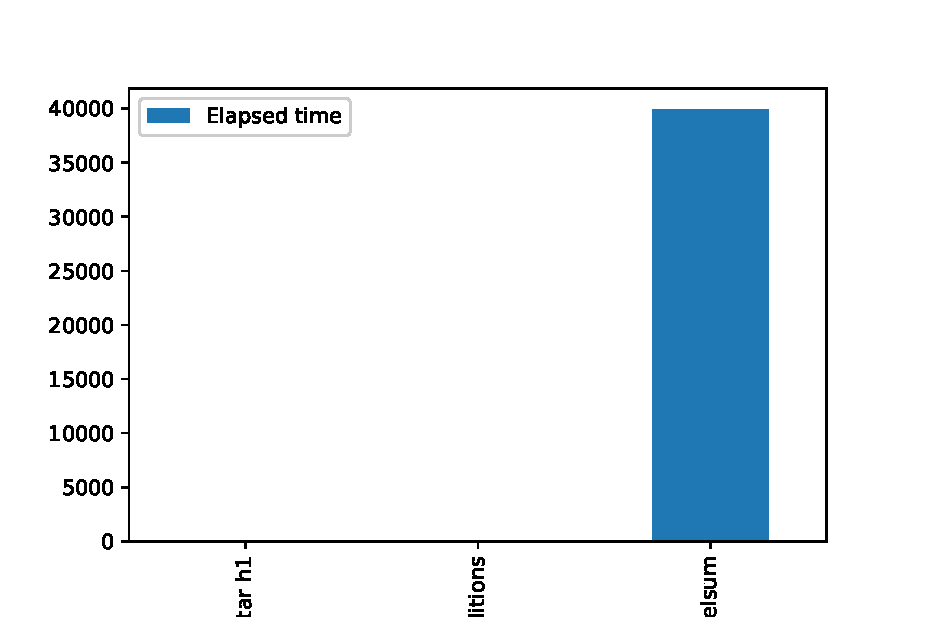
\includegraphics{astarp3.eps}
  \caption{A-star comparison of h1, ignore preconditions and level-sum heuristics}
  \label{fig:astarp3}
\end{figure}

The ignore preconditions heuristic, as described in \cite{russell1995modern} chapter 11, p. 386,
is an admissible heuristic and is very simple to compute, but not very accurate.
The level-sum heuristic (admissible if sub-goals are independent) is much more accurate.


\subsection{Closing remarks}

The uninformed search methods performed better in terms of elapsed time than the A-star
algorithm, no matter what heuristic was selected. The expected result would be that
the level-sum heuristic would outperform all other methods, because of the smallest number
of nodes expanded and goal tests, however due to inneficiency of the implementation - it took
the longest to compute. The winning algorithm, in terms of speed, is DFS, however it does not guarantee
an optimal solution.

\printbibliography

\end{document}
